\subsection{Motivations}

\begin{itemize}
    \item RNNs were the state of the art for sequence in sequence modeling, as they rely on the 
        generation of hidden states $h^{(t)}$ as a function of the previous one $h^{(t-1)}$ and the 
        input $x^{(t)}$ \uB{they cannot be trained in with parallelization paradigm}.
    \item Attention mechanism gained a lot in relevancy as it allows \uB{modeling dependencies 
            regardless the position} in input and output sequences.
\end{itemize}

Finally why do not build an architecture relying only on this interesting attention mechanism ?

\subsection{Encoder and Decoder stacks}

\begin{figure}[H]
    \begin{center}
        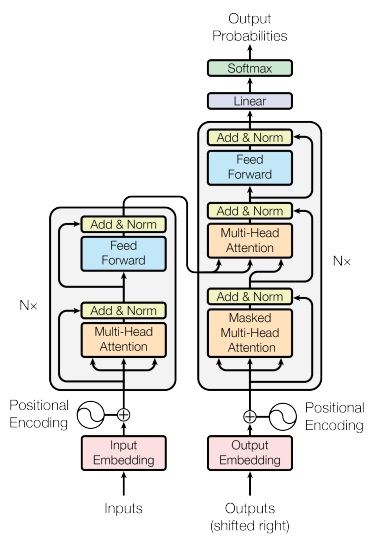
\includegraphics[width=.5\textwidth]{chapters/4_deep_learning/3_types_of_neural_networks/images/05_transformer_model_architecture.png}
    \end{center}
    \caption{Transformer model architecture}
    \label{fig:05_transformer_model_architecture}
\end{figure}

\paragraph{Encoder}


It is \tB{composed of $N$ (initially $N=6$) identical layers}, each one has two sub-layers:
\begin{enumerate}
    \item multi-head self-attention mechanism
    \item simple position-wise (meaning independently applied to each element of the sequence)\\
        $FFN(x) = \max\left(0, xW_{1} + b_{1}\right)W_{2} + b_{2}$
\end{enumerate}

\uB{A residual connection is employed around each of these two sub-layers} followed by a layer 
normalization, that is each of them has as output: $LayerNorm\left(x + Sublayer(x)\right)$

\paragraph{Decoder}
Decoder relies on the same principle except that it contains a \tB{third sub-layer performing 
multi-head attention over the output of the encoder} stack. It is worth noting that self-attention 
sub-layer has been modified to \uB{prevent positions from attending to subsequent positions}, more 
precisely it is a masking. The output embedding are offset by one position ensuring that position $i$
can only depends on position $j$ such that $j\leq i$.


\subsection{Attention}

An \emph{attention mechanism} can be described as mapping a \tB{query} and a set of \tB{key-value 
pairs} to an output, note that \uB{query, keys, values and output are all vectors}.\
The output is a weighting sum of the values, while \tR{the weight associate to each of these values 
reflects the compatibility between the query and the key of the considered value}. \
Consider a sequence of length $n$, and 
Let $d_{k}$, $d_{v}$ and $d_{model}$ be the dimensions of the keys, the values and the vector 
(usually 512)
representation.

\paragraph{Scaled Dot-Product Attention}

We compute the matrix: 
\begin{center}
    \fr{$Attention\left(\bm{Q},\bm{K},\bm{V}\right)=\text{softmax}\left(\dfrac{\bm{Q}\bm{K}^{T}}{\sqrt{d_{k}}}\right)\bm{V}$}
\end{center}

Step by step:

\begin{itemize}
    \item For an input $X\in\mathcal{M}(\mathbb{R})_{n,d_{model}}$ then:
        \begin{itemize}
            \item $Q = XW_{Q}$ projection matrix $W_{Q} \in\mathcal{M}(\mathbb{R})_{d_{model},d_{k}}$
            \item $K = XW_{K}$ projection matrix $W_{K} \in\mathcal{M}(\mathbb{R})_{d_{model},d_{k}}$
            \item $V = XW_{V}$ projection matrix $W_{V} \in\mathcal{M}(\mathbb{R})_{d_{model},d_{v}}$
        \end{itemize}
        
    \item $QK^{T} \in\mathcal{M}(\mathbb{R})_{n,n}$ where the element located at $(i, j)$ represents
        \uR{how much position $i$ \emph{attends to} position $j$}.
    \item scaling by $\sqrt{d_{k}}$ is justified by the fact for large values of $d_{k}$ the dot 
        products grow large in magnitude pushing the softmax into regions where it has extremely 
        small gradients
    \item applying softmax function row-wise to transform each row into a probability distribution
    \item multiplying by $V$ resulting in a matrix $\mathcal{M}(\mathbb{R})_{n,d_{v}}$, where the 
        element located at \tR{$(i, l)$ represents the weighted average of all the positions at the
        $l^{th}$ representation dimension (of matrix $V$) from the perspective of the $i^{th}$ 
        position}.\
        We talk about weighted average and not just weighted sum because the weights constitute a 
        probability distribution of attention score associated with the $i^{th}$ position.
\end{itemize}


\paragraph{Multi-Head Attention}

It has been found more beneficial to avoid using a single attention function (or head) with 
$d_{model}$ dimensional keys, values and queries and thus repeat the process of scaled-dot product 
attention $h$ (usually $h=8$) times in parallel with different projection matrices.
Originally $d_{v}=d_{k}=\frac{d_{model}}{h} = 64$

\begin{center}
    \fr{$MultiHead\left(\bm{Q},\bm{K},\bm{V}\right) = Concat\left(\left(head_i\right)_{1\leq i\leq h}\right)P^{O}$}
\end{center}

Note that $head_{i} = Attention\left(\bm{Q}\bm{P}_{i}^{Q},\bm{K}\bm{P}_{i}^{K},\bm{V}\bm{P}_{i}^{V}\right)$ and
$
\begin{cases}
\bm{P}_{i}^{Q}\in\mathcal{M}(\mathbb{R})_{d_{model},d_{k}}\\
\bm{P}_{i}^{K}\in\mathcal{M}(\mathbb{R})_{d_{model},d_{k}}\\ 
\bm{P}_{i}^{V}\in\mathcal{M}(\mathbb{R})_{d_{model},d_{v}}\\
\bm{P}_{i}^{Q}\in\mathcal{M}(\mathbb{R})_{h\times d_{v},d_{model}}
\end{cases}
$

The final projection allows the heads to interact and combine their information.
